\documentclass{article}

\usepackage{amsmath,amssymb}
\usepackage{geometry}
\usepackage{graphicx}

\geometry{a4paper, margin=2.5cm}

\begin{document}

% ============================================================
\section*{The Multi-Armed Bandit Problem (MAB)}

\subsection*{First, a story}

You walk into a casino facing $K$ slot machines. Each machine has its own winning probability, but you know none of them. You have $T$ pulls (one coin each) and want to maximize your total payout.

\textbf{The core dilemma}: which machine do you feed your coins?
\begin{itemize}
  \item Play the one that \emph{looks} good --- you may be misled by early luck and forever miss the truly best machine;
  \item Try every machine --- pulling the bad ones is pure waste.
\end{itemize}

This is the \textbf{exploration vs.\ exploitation} trade-off, the wellspring of every problem in reinforcement learning.

\subsection*{Formalization}

A $K$-armed Bernoulli bandit is defined by:

\[
\boxed{\text{Bandit}_K = \{\mu_1, \mu_2, \ldots, \mu_K\}, \quad \mu_k \in [0,1]}
\]

\begin{itemize}
  \item $\mu_k$ --- the true winning probability of arm $k$ (\textbf{unknown});
  \item action $a_t \in \{1,\ldots,K\}$ --- which arm to pull at step $t$;
  \item reward $r_t \in \{0,1\}$ --- the realized payout, $r_t \sim \text{Bernoulli}(\mu_{a_t})$;
  \item optimal arm $\mu^* = \max_k \mu_k$, with index $k^* = \arg\max_k \mu_k$.
\end{itemize}

Objective: over $T$ steps, choose the action sequence $(a_1,\ldots,a_T)$ that maximizes expected cumulative reward $\mathbb{E}\left[\sum_{t=1}^{T} r_t\right]$.

% ============================================================
\section*{Regret --- the yardstick for algorithms}

\subsection*{Definition}

Maximizing reward is equivalent to minimizing \textbf{regret} --- how much you lose for not knowing the best arm.

If step $t$ pulls arm $a_t$, the \textbf{instantaneous regret} is:
\[
\boxed{\rho_t = \mu^* - \mu_{a_t}}
\]

and the \textbf{cumulative regret} after $T$ steps:
\[
\boxed{R(T) = \sum_{t=1}^{T} \rho_t = T\mu^* - \sum_{t=1}^{T} \mu_{a_t}}
\]

\subsection*{What regret tells us}

\[
\begin{array}{c|c}
\text{Growth rate of regret} & \text{Meaning} \\
\hline
R(T) = O(T) \;\; \text{(linear)} & \text{the algorithm is not learning --- it keeps making mistakes} \\
R(T) = O(\log T) \;\; \text{(logarithmic)} & \text{the algorithm is learning --- mistakes grow ever rarer} \\
R(T) = O(\sqrt{T}) \;\; \text{(square root)} & \text{in between the two} \\
\end{array}
\]

\textbf{The Lai \& Robbins lower bound (1985)}: any uniformly good algorithm (sublinear regret on every instance) incurs at least $\Omega(\log T)$. Note that $O(\log T)$ is only rate-optimal; matching the constant of the bound ($\sum_k \Delta_k / \mathrm{KL}(\mu_k,\mu^*)$) is what asymptotic optimality means.

% ============================================================
\section*{Greedy and $\varepsilon$-greedy}

\subsection*{Purely greedy}

The most naive idea: always pull the arm with the best current estimate.
\[
a_t = \arg\max_k \hat{\mu}_k(t), \qquad
\hat{\mu}_k(t) = \frac{\text{total reward collected from arm } k}{\text{number of times arm } k \text{ was pulled}}
\]

\textbf{Fatal flaw}: the first time a suboptimal arm happens to pay out $r=1$, it is estimated at $\hat{\mu}_k = 1.0$. Pure greedy then never touches another arm again --- it is stuck on a suboptimal choice forever, and regret grows linearly.

\subsection*{$\varepsilon$-greedy}

\textbf{Core idea}: exploit greedily most of the time; explore uniformly with a small probability.

\[
a_t = \begin{cases}
  \text{choose } k \in \{1,\ldots,K\} \text{ uniformly}, & \text{with probability } \varepsilon \text{ (explore)},\\[4pt]
  \arg\max_k \hat{\mu}_k(t), & \text{with probability } 1-\varepsilon \text{ (exploit)}.
\end{cases}
\]

\subsection*{The incremental mean update (important!)}

There is no need to store the full reward history. Given $N$ observations with mean $\hat{\mu}_N$, a new observation $r_{N+1}$ updates:
\[
\begin{aligned}
\hat{\mu}_{N+1} &= \frac{1}{N+1}\sum_{i=1}^{N+1} r_i
                 = \frac{1}{N+1}\left(r_{N+1} + \sum_{i=1}^{N} r_i\right) \\[4pt]
                &= \frac{1}{N+1}\left(r_{N+1} + N\hat{\mu}_N\right) \\[4pt]
                &= \frac{1}{N+1}\left(r_{N+1} + (N+1)\hat{\mu}_N - \hat{\mu}_N\right) \\[4pt]
                &= \hat{\mu}_N + \frac{1}{N+1}\left(r_{N+1} - \hat{\mu}_N\right).
\end{aligned}
\]

\[
\boxed{\hat{\mu}^{\text{new}} = \hat{\mu}^{\text{old}} + \frac{1}{N+1}\left(r - \hat{\mu}^{\text{old}}\right)}
\]

\textbf{Why this form matters}: it is the prototype of \underline{every update rule in RL}:
\[
\theta \leftarrow \theta + \alpha\,(\text{Target} - \theta)
\]
Q-Learning's $Q(s,a) \leftarrow Q(s,a) + \alpha\,(r + \gamma\max Q - Q(s,a))$ is exactly this structure.

\subsection*{Regret analysis of constant $\varepsilon$}

With fixed $\varepsilon > 0$, each step selects any specific arm with probability $\varepsilon/K$. A suboptimal arm $k$ is explored in expectation $\frac{\varepsilon}{K}T$ times over $T$ steps, each pull costing regret $\Delta_k = \mu^* - \mu_k$:

\[
\mathbb{E}[R(T)] \ge \sum_{k: \Delta_k > 0} \frac{\varepsilon}{K}\,T \cdot \Delta_k = \frac{\varepsilon}{K}\,T\sum_k \Delta_k = \Omega(T)
\]

\textbf{Conclusion}: a constant $\varepsilon$ gives linear regret --- even as $T \to \infty$, exploration never stops and keeps wasting pulls.

\subsection*{Decaying $\varepsilon$-greedy}

\textbf{Improvement}: let the exploration probability decay over time. With $\varepsilon_t = 1/t$:
\[
\mathbb{P}(\text{explore at step } t) = \frac{1}{t} \;\longrightarrow\; 0 \quad (t \to \infty)
\]

Heavy exploration early (large $\varepsilon_t$ for small $t$), focused exploitation late. A rigorous logarithmic-regret guarantee needs a sufficiently large decay constant: taking $\varepsilon_t = cK/(d^2t)$ ($d$ the minimum suboptimality gap, Auer et al.\ 2002) yields $O(\log T)$ regret; plain $\varepsilon_t = 1/t$ only guarantees sublinear regret, and matches the rate rather than the lower-bound constant.

\textbf{Caveat}: the total number of explorations under $\varepsilon_t = c/t$ is about $c\ln T$; if $c$ is too small (e.g., $c=1$), there is barely any exploration within a finite horizon. In practice one often imposes a floor $\varepsilon_{\min}$ (such as $0.02$) to retain enough exploration (see Figure~\ref{fig:optimal-arm}).

\subsection*{Optimistic initialization}

Another exploration-inducing trick: initialize all estimates at $1.0$ (the maximum possible). Every arm starts overestimated --- pulling an arm lowers its estimate while the others stay ``inflated'', forcing the algorithm to try them all. A round of exploration happens naturally, then the algorithm converges to greedy.

% ============================================================
\section*{Upper Confidence Bound (UCB)}

\subsection*{The problem with $\varepsilon$-greedy}

Its exploration is \textbf{undirected} --- it picks uniformly among all arms, wasting pulls on obviously bad ones. Good exploration should be directed: ``I am uncertain about this arm, so let me try it.''

\subsection*{Core idea: optimism in the face of uncertainty}

UCB looks beyond the point estimate $\hat{\mu}_k$ and computes a \textbf{confidence upper bound}. The more uncertain an arm, the higher its bound gets pushed --- even a mediocre point estimate can win selection because ``it might be great''.

\[
\boxed{a_t = \arg\max_k \left[\; \hat{\mu}_k(t) \;+\; \text{uncertainty bonus} \;\right]}
\]

\subsection*{Hoeffding's inequality --- quantifying uncertainty}

Let $X_1,\ldots,X_n$ be i.i.d.\ random variables in $[0,1]$ with $\bar{X}_n = \frac{1}{n}\sum_i X_i$ and $\mu = \mathbb{E}[X_i]$:

\[
\boxed{\mathbb{P}\left(|\bar{X}_n - \mu| \ge \delta\right) \le 2\exp\left(-2n\delta^2\right)}
\]

\textbf{In plain words}: after $n$ observations, the probability that the sample mean deviates from the true expectation by $\ge \delta$ shrinks exponentially.

Run the inequality backwards: given confidence level $p$, solve $\exp(-2n\delta^2)=p$:
\[
\delta = \sqrt{\frac{\log(1/p)}{2n}}
\]

Taking $p = 1/t$ (tightening confidence as time goes on), with probability $\ge 1-2/t$:
\[
\mu_k \in \left[\hat{\mu}_k - \sqrt{\frac{\log t}{2 N_k}},\; \hat{\mu}_k + \sqrt{\frac{\log t}{2 N_k}}\right]
\]

Select the \textbf{upper bound} (the optimistic estimate):
\[
\boxed{a_t = \arg\max_k \left[\; \underbrace{\hat{\mu}_k(t)}_{\text{exploit}} \;+\; \underbrace{c \cdot \sqrt{\frac{\log t}{2\,N_k(t)}}}_{\text{exploration bonus}} \;\right]}
\]

\textbf{Intuition}:
\begin{itemize}
  \item a heavily pulled arm ($N_k$ large) $\to$ small bonus $\to$ the bound tightens;
  \item a neglected arm ($N_k$ small) $\to$ large bonus $\to$ the bound inflates $\to$ it gets selected again;
  \item $\log t$ grows so slowly with $t$ that the long-run exploration cost stays small.
\end{itemize}

$c$ is a hyperparameter trading off exploration and exploitation. Implementations usually smooth $N_k$ (e.g., $N_k+1$) to avoid division by zero and to give unpulled arms maximal uncertainty, ensuring every arm is tried at least once.

\subsection*{Regret upper bound (Auer et al.\ 2002)}

UCB1 ($c=1$) guarantees:
\[
\mathbb{E}[R(T)] \le 8\sum_{k: \mu_k < \mu^*} \frac{\log T}{\Delta_k} + C, \quad \text{i.e., } O(\log T)
\]
which is asymptotically optimal in rate. Each suboptimal arm is pulled in expectation $\approx \frac{\log T}{\Delta_k^2}$ times before its confidence interval is too narrow to compete; afterwards it is all but forgotten.

% ============================================================
\section*{Thompson Sampling}

\subsection*{Frequentist vs.\ Bayesian}

The first three algorithms (Greedy, $\varepsilon$-Greedy, UCB) take a \textbf{frequentist} view: compute a point estimate $\hat{\mu}_k$ from history, then add something around it (noise / confidence bounds).

Thompson Sampling is \textbf{Bayesian}: instead of maintaining ``one number'', maintain the \textbf{full probability distribution} of $\mu_k$ --- expressing ``what I believe about $\mu_k$''.

\subsection*{The Beta distribution and conjugate priors}

The likelihood of Bernoulli trials (having observed $s$ successes and $f$ failures):
\[
P(\text{data} \mid \mu) = \mu^{s}\,(1-\mu)^{f}
\]

The Beta density:
\[
\text{Beta}(\theta \mid \alpha, \beta) \propto \theta^{\alpha-1}(1-\theta)^{\beta-1}, \quad \theta \in [0,1]
\]

The two share the same functional form (a power of $\mu$ times a power of $(1-\mu)$). Hence:

\textbf{if the prior is Beta, then after seeing Bernoulli data the posterior is again Beta} (conjugacy):

\[
\boxed{P(\mu \mid s \text{ successes, } f \text{ failures}) = \text{Beta}(\alpha_0 + s,\; \beta_0 + f)}
\]

With $\alpha_0 = \beta_0 = 1$, $\text{Beta}(1,1) = \text{Uniform}(0,1)$ --- ``I know nothing''.

\subsection*{From prior to posterior}

\[
\begin{aligned}
P(\mu \mid r_{1:n}) &\propto P(r_{1:n} \mid \mu) \cdot P(\mu)  \\
&\propto \mu^{\sum r_i} (1-\mu)^{n-\sum r_i} \cdot \mu^{\alpha_0-1} (1-\mu)^{\beta_0-1} \\
&= \mu^{\alpha_0 + \sum r_i - 1}\,(1-\mu)^{\beta_0 + n - \sum r_i - 1} \\
&\propto \text{Beta}\left(\alpha_0 + \sum r_i,\; \beta_0 + n - \sum r_i\right).
\end{aligned}
\]

\textbf{How the Beta distribution evolves with data}:

\[
\begin{array}{c|c|c}
\text{Parameters} & \text{Meaning} & \text{Shape} \\
\hline
\alpha=1,\;\beta=1     & \text{uninformative prior} & \text{uniform } U[0,1] \\
\alpha=10,\;\beta=10   & 9\ \text{wins},\ 9\ \text{losses} & \text{concentrated near } 0.5 \text{, wide} \\
\alpha=80,\;\beta=20   & 79\ \text{wins},\ 19\ \text{losses} & \text{concentrated near } 0.8 \text{, narrow} \\
\alpha=200,\;\beta=50  & 199\ \text{wins},\ 49\ \text{losses} & \text{concentrated near } 0.8 \text{, narrower (very confident)} \\
\end{array}
\]

More data, narrower distribution --- the belief about $\mu_k$ becomes more certain.

The experimental view of posterior convergence under Thompson Sampling is shown in Figure~\ref{fig:thompson-posterior}.

\begin{figure}[!htbp]
  \centering
  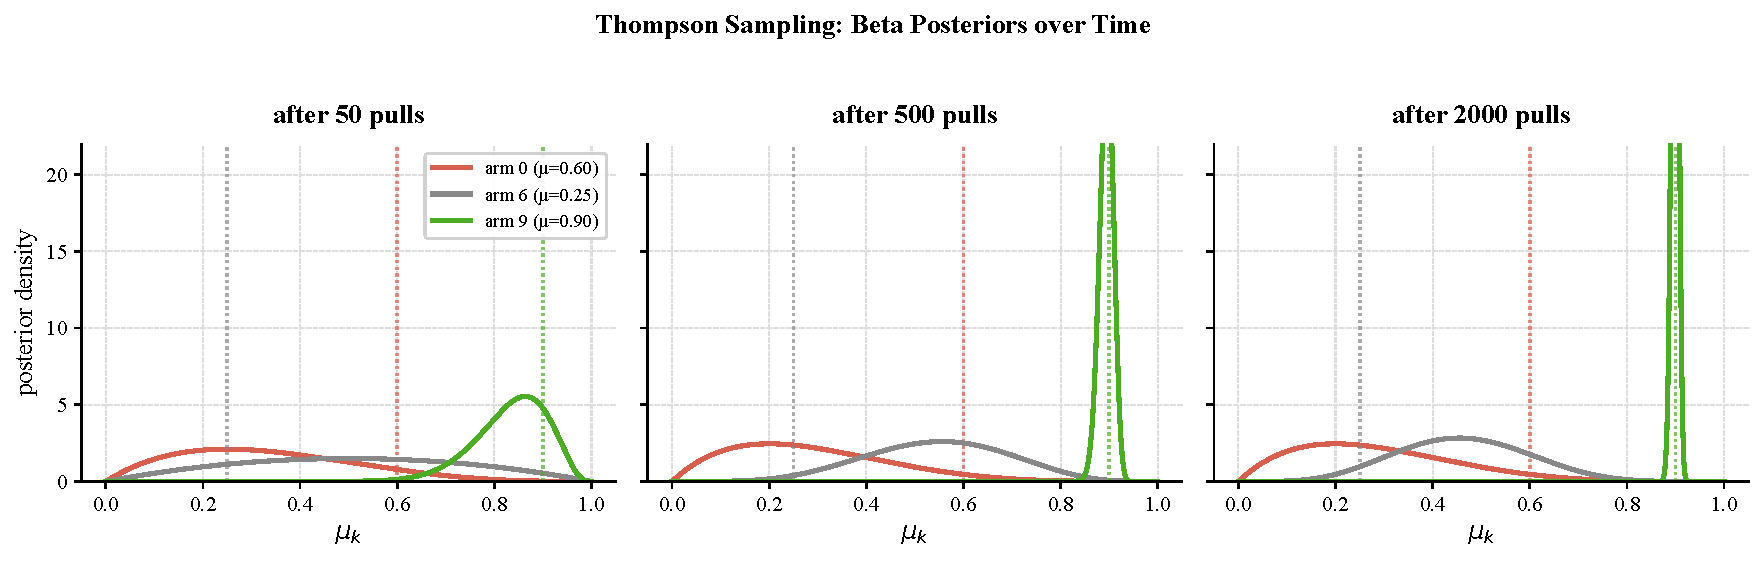
\includegraphics[width=0.92\textwidth]{fig3_thompson_posterior.pdf}
  \caption{Posterior evolution under Thompson Sampling (10-armed Bernoulli bandit, optimal arm $\mu^*=0.90$, fixed seed). Posteriors $\mathrm{Beta}(\alpha_k,\beta_k)$ of three arms at three moments (steps 50 / 500 / 2000): the optimal arm (green) is pulled heavily and its posterior tightens rapidly around $0.90$; a neglected suboptimal arm (gray) stays wide --- posterior width is exactly what drives exploration in Thompson Sampling. Dotted lines mark the true $\mu_k$ of each arm.}
  \label{fig:thompson-posterior}
\end{figure}

\subsection*{The algorithm: three lines}

\begin{enumerate}
  \item \textbf{Sample}: draw one sample $\tilde{\mu}_k \sim \text{Beta}(\alpha_k, \beta_k)$ from each arm's posterior;
  \item \textbf{Select}: $a_t = \arg\max_k \tilde{\mu}_k$ (greedy on the samples);
  \item \textbf{Update}: $\alpha_{a_t} \leftarrow \alpha_{a_t} + r_t$, $\beta_{a_t} \leftarrow \beta_{a_t} + (1 - r_t)$.
\end{enumerate}

\subsection*{Why does ``sample from the posterior, then act greedily'' work?}

\textbf{Probability matching}: the probability of selecting arm $k$ equals the posterior probability that arm $k$ is the best:
\[
\mathbb{P}(a_t = k) = \mathbb{P}\big(\mu_k = \max_j \mu_j \,\big|\, \text{data}\big)
\]

\textbf{Exploration and exploitation balance automatically}:
\begin{itemize}
  \item an uncertain arm (wide Beta) $\to$ its sample swings widely, sometimes very high $\to$ it naturally gets exploration;
  \item a confidently bad arm (narrow Beta concentrated low) $\to$ almost never samples above a good arm $\to$ little waste.
\end{itemize}

\subsection*{Regret analysis (Agrawal \& Goyal 2012)}

Thompson Sampling also achieves expected cumulative regret $O(\log T)$; for the Bernoulli case, Kaufmann, Korda \& Munos (2012) further proved that its asymptotic constant matches the Lai \& Robbins lower bound. In practice it is usually the strongest performer.

% ============================================================
\section*{Comparing the four algorithms}

Experiments (Figures~\ref{fig:regret} and \ref{fig:optimal-arm}): a 10-armed Bernoulli bandit, 20 random seeds --- each algorithm behaves exactly as the theory predicts.

\begin{figure}[!htbp]
  \centering
  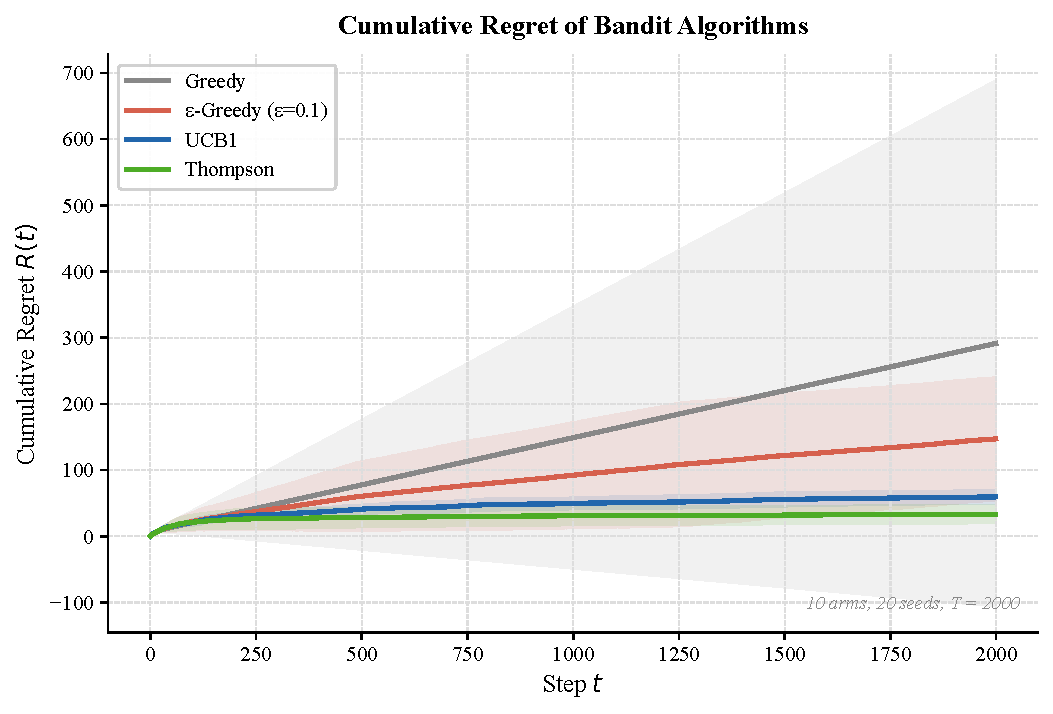
\includegraphics[width=0.88\textwidth]{fig1_regret_comparison.pdf}
  \caption{Cumulative regret $R(T)$ of the four algorithms (20 random seeds, shading $\pm 1\sigma$). Greedy grows nearly linearly; $\varepsilon$-Greedy ($\varepsilon=0.1$) is next but still linear; UCB and Thompson Sampling are sublinear ($O(\log T)$).}
  \label{fig:regret}
\end{figure}

\subsection*{How the exploration styles differ}

\begin{itemize}
  \item \textbf{$\varepsilon$-Greedy}: undirected random exploration. ``The rule says explore, so I explore.''
  \item \textbf{UCB}: directed exploration. ``I'm uncertain about arm B --- what if it's great? Give it a chance.''
  \item \textbf{Thompson Sampling}: probabilistic exploration. ``I believe arm B has a 30\% chance of being best, so I pick it 30\% of the time.''
  \item \textbf{Decaying $\varepsilon$-Greedy}: same family as $\varepsilon$-Greedy, with a decaying exploration rate.
\end{itemize}

The fraction of pulls given to the optimal arm also exposes these differences, as shown in Figure~\ref{fig:optimal-arm}.

\begin{figure}[!htbp]
  \centering
  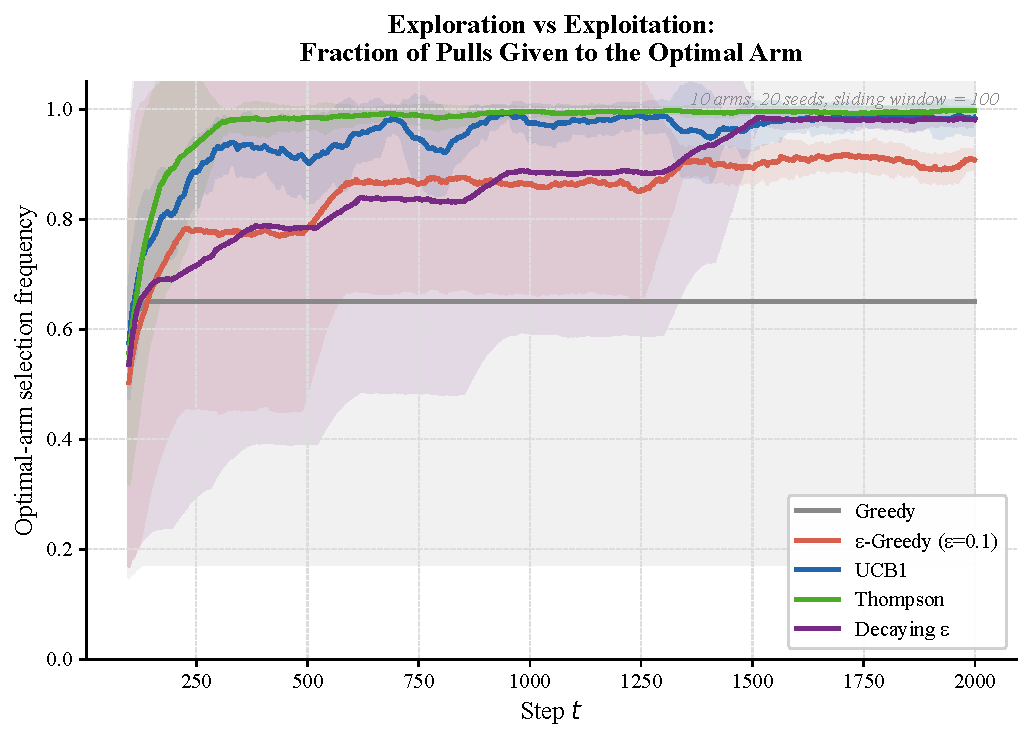
\includegraphics[width=0.88\textwidth]{fig2_optimal_arm_selection.pdf}
  \caption{Fraction of pulls on the optimal arm (20 random seeds, 100-step moving average, shading $\pm 1\sigma$). Greedy locks onto a single arm per seed --- here about three in ten seeds get stranded on a suboptimal arm; $\varepsilon$-Greedy plateaus near $1-\varepsilon=0.9$; decaying $\varepsilon$ climbs slowly toward 1; UCB and Thompson Sampling converge fastest.}
  \label{fig:optimal-arm}
\end{figure}

\subsection*{One table to rule them all}

\begin{center}
\small
\begin{tabular}{c|c|c|c}
\textbf{Algorithm} & \textbf{Exploration} & \textbf{Regret} & \textbf{Notes} \\
\hline
$\varepsilon$-Greedy & uniformly random & $O(T)$ (linear) & simplest; regret never converges \\
Decaying-$\varepsilon$ & random, decaying & $O(\log T)$ (needs tuned $c$) & a simple improvement \\
UCB & directed (bounds) & $O(\log T)$ & deterministic, few knobs \\
Thompson Sampling & directed (sampling) & $O(\log T)$, optimal constant & strongest in practice \\
\end{tabular}
\end{center}

\subsection*{Practical recommendations}

\begin{enumerate}
  \item Rapid prototyping / teaching: $\varepsilon$-Greedy or Decaying $\varepsilon$-Greedy.
  \item Theoretical guarantees with few knobs: UCB (a single parameter $c$).
  \item Real applications (recommender systems, ad serving, A/B testing): \textbf{Thompson Sampling} --- usually the best performer, and priors let domain knowledge flow in naturally.
\end{enumerate}

% ============================================================
\section*{Where this chapter sits in the RL landscape}

The MAB is single-state reinforcement learning. Understanding it gives you the seed of three core RL concepts:

\begin{enumerate}
  \item \textbf{Exploration vs.\ exploitation} --- the MAB is its purest form; in an MDP it becomes ``which state--action pair to explore'', an isomorphic question.
  \item \textbf{Incremental updates} $\theta \leftarrow \theta + \alpha(\text{Target} - \theta)$ --- the shared update skeleton of TD learning, Q-Learning, and Policy Gradient.
  \item \textbf{Uncertainty-driven exploration} --- UCB $\to$ count-based exploration $\to$ RND (Random Network Distillation); Thompson Sampling $\to$ PSRL (Posterior Sampling RL), the gateway to Bayesian RL.
\end{enumerate}

The next chapter, MDPs, extends ``single state'' to ``state transitions''; with the Markov property and the Bellman equations, the theoretical edifice of RL stands complete.

\subsection*{References}

\begin{enumerate}
  \item Sutton \& Barto (2018). \textit{Reinforcement Learning: An Introduction} (2nd ed.). Chapter 2.
  \item Lai \& Robbins (1985). Asymptotically efficient adaptive allocation rules. \textit{Advances in Applied Mathematics}.
  \item Auer, Cesa-Bianchi \& Fischer (2002). Finite-time analysis of the multiarmed bandit problem. \textit{Machine Learning}.
  \item Agrawal \& Goyal (2012). Analysis of Thompson sampling for the multi-armed bandit problem. \textit{COLT}.
  \item Kaufmann, Korda \& Munos (2012). Thompson Sampling: An Asymptotically Optimal Finite-Time Analysis. \textit{ALT}.
  \item Hands-on RL (\textit{Dongshou Xueqianghua Xuexi}, Chinese). Chapter 2: multi-armed bandits.
\end{enumerate}

\end{document}
